\documentclass{ansconf}

\usepackage[T1]{fontenc}     % Use T1 encoding instead of OT1
\usepackage[utf8]{inputenc}  % Use UTF8 input encoding
\usepackage{microtype}       % Improve typography
\usepackage{amsmath}         % AMS Math extensions
\usepackage{booktabs}        % Improved table spacing
\usepackage{graphicx}
\usepackage{url}

\authorHead{Romano et al.}
\shortTitle{Progress and Status of OpenMC}
\confTitle{International Conference on Mathematics and Computational Methods
  Applied to Nuclear Science \& Engineering (M\&C 2013)}
\confLocation{Sun Valley, Idaho, USA, May 5-9, 2013}
\confPublished{on CD-ROM, American Nuclear Society, LaGrange Park, IL (2013)}

\begin{document}

\title{Progress and Status of the OpenMC Monte Carlo Code}

\author{Paul K. Romano}
\author{Bryan R. Herman}
\author{Nicholas E. Horelik}
\author{Benoit Forget}
\author{Kord Smith}
\affil{Massachusetts Institute of Technology  \\
  Department of Nuclear Science and Engineering \\
  77 Massachusetts Avenue, Cambridge, MA 02139 \\
  paul.romano@alum.mit.edu; bherman@mit.edu; nhorelik@mit.edu; bforget@mit.edu;
  kord@mit.edu}

\author{Andrew R. Siegel}
\affil{Argonne National Laboratory  \\
  Theory and Computing Sciences and Nuclear Engineering Division \\
  siegela@mcs.anl.gov
}

\maketitle

\begin{abstract}
The present work describes the latest advances and progress in the development
of the OpenMC Monte Carlo code, an open-source code originating from the
Massachusetts Institute of Technology. First, an overview of the development
workflow of OpenMC is given. Various enhancements to the code and user input
such as real-time validation are described.

\emph{Key Words}: Monte Carlo, transport, open source, OpenMC
\end{abstract}

\section{Introduction}

With the continual improvement of high-performance computing, many in the
reactor physics community have begun to envision a future in which Monte Carlo
methods could be used for the simulation of large light-water reactors. While
possessing a number of inherent advantages over deterministic methods, the fact
of the matter is that there are many challenges to be overcome before Monte
Carlo methods realistically could be used in commercial reactor analysis
\cite{net-martin-2012}. A great deal of research and development efforts are now
focused on addressing some of these outstanding issues.

The Computational Reactor Physics Group at MIT has for the last few years
focused on analyzing and developing solutions to some of the algorithmic
problems that have been an impediment to successful large-scale parallel Monte
Carlo simulations \cite{pnst-romano-2011, nse-romano-2012,
  trans-romano-2012}. In addition, a collaboration with Argonne National
Laboratory under the Center for Exascale Simulation of Advanced Reactors has
helped to advance the theoretical understanding of domain and data decomposition
algorithms \cite{jcp-siegel-2012-1, jcp-siegel-2012-2}. All of these efforts
were made possible by the development of a modern Monte Carlo particle transport
code, OpenMC \cite{openmc-github-2012}.

The basic geometry and physics algorithms in OpenMC have been described in
detail previously \cite{ane-romano-2012}. In the present work, we seek to shed
light on some of the more recent developments within the OpenMC community with a
particular focus on the software development workflow that has enabled high
productivity development and encouraged participation by individuals and
organizations outside of the immediate reactor physics community at MIT.

\section{Development}

Having grown from a single developer at the beginning of 2011 to numerous
developers across multiple institutions, the future success of OpenMC will
strongly depend on a productive workflow. Traditionally, the development of
software within the nuclear industry has been carried out within single
institutions. To the authors' knowledge, there have not been many
multi-organization collaborative software development efforts. In many cases,
there is good reason for this --- maintaining effective management of a project
that many organizations are contributing to can be fraught with difficulty. On
top of that, the open-source model introduces unique complexities into the
software development process; who decides what ultimately goes into the
``official'' version? How is work delegated among developers scattered across
the globe?  In his famous essay ``The Cathedral and the Bazaar'', Eric Raymond
noted the challenges of open-source projects, remarking that \cite{raymond-1999}
open-source communities sometimes ``resemble a great babbling bazaar of
differing agendas and approaches ... out of which a coherent and stable system
could seemingly emerge only by a succession of miracles.'' Despite these
challenges, open-source projects can and often do thrive when an enthusiastic
development community coalesces. Indeed, even at this early stage, we have
received unsolicited contributions and bug-fixes from user/developers outside of
MIT.

The decision to release OpenMC as open-source software and encourage
participation from outsiders is predicated on the assumption that doing so will
be mutually beneficially both to the originating community (MIT) and those who
adopt the code for further development. It is our hope and belief that by
embracing open collaboration, researchers at different institutions can more
effectively work towards a common goal rather than compete with one another.

\subsection{Collaboration Workflow}

Internally, we have adopted an integration-manager workflow as described by
Chacon \cite{chacon-2009}. This workflow works particularly well with the GitHub
hosting service that is used by OpenMC. On GitHub, each developer can easily
fork a project creating their own public copy of the OpenMC repository. They are
then free to make whatever changes and modifications they wish; note that they
are not required to have any special access on the original repository. If a
developer wants their changes to be merged into the official project, they can
issue a \emph{pull request} --- at this point, the person designated as the
integration manager then reviews the request and, if the changes are acceptable,
merges it in.

One of the early concerns raised by a number of developers was the ability to
keep some work private even though the project as a whole is open-source. The
motivation for privacy could be unpublished research that is not ready to be
shared, patentable ideas, commercial ideas, etc. A developer who wishes to have
a private copy of OpenMC can do so either by having a local copy on their
machine with a remote reference set up to the main OpenMC repository so that
they can still pull updates. Another option is to maintain a private copy on
GitHub. The general integration-manager workflow is shown in the diagram in
Figure \ref{fig:workflow}. The dashed lines represent \emph{pulls} whereas solid
lines indicate \emph{pushes}. At MIT, work is carried out on branches (indicated
by yellow boxes) of the main repository, public forks, and private copies
depending on the nature of the development.

\begin{figure}[!htb]
  \centering
  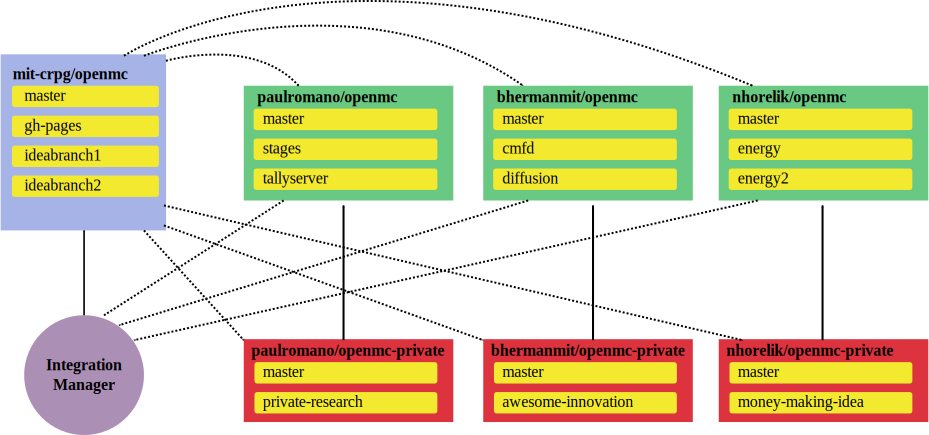
\includegraphics[width=6.5in]{integration-manager}
  \caption{Integration manager workflow pattern used in OpenMC development.}
  \label{fig:workflow}
\end{figure}

\subsection{Real-time XML Validation}

OpenMC uses an XML syntax for all user input and configuration files. The use of
XML is of great benefit to both developers and users. Developers can make
changes to the user input format easily, adding or modifying options, and the
xml-fortran parser within OpenMC gracefully handles the changes with little
effort from the developer. Users are free to form their input files as they
like, as long as the overall structure of the files is well-formed and the
content conforms to the specification of the file.  Until recently, it was only
possible to check that user input files were well-formed prior to running,
i.e. content was defined, properly delimited with a start and end tag, and
properly nested. A set of schemata based on the RELAX NG schema language
\cite{relaxng-2008} has now made it possible to check not only that an input
file is well-formed but also that it has the correct tags, attributes, and
datatypes.

At present, there are two ways that input files can be checked for conformance
against the schemata. The first method is post-validation where once an input
file has been written, it is checked against a corresponding schema using a tool
such as \texttt{jing}. From a command-line, the user could enter \texttt{jing -c
  \textasciitilde/openmc/src/templates/geometry.rnc geometry.xml} and any errors
in the input file would be reported back. The first argument is the
corresponding schema and the second argument is the XML input file. A more
elegant method to check conformance is real-time validation with an editor such
as GNU Emacs. When using GNU Emacs to write an input file, the input is
continually checked against a corresponding schema (based on the root element in
the document). If any errors are found, they are highlighted in red giving the
user immediate visual feedback. Figure \ref{fig:relaxng} shows an example of an
input file being validated against a schema in GNU Emacs.

\begin{figure}[!htb]
  \centering
  \includegraphics[width=5.0in]{relaxng.png}
  \caption{Example of an XML input file in GNU Emacs being validated against a
    corresponding RELAX NG schema in real-time. Errors in the input are
    automatically highlighted in red.}
  \label{fig:relaxng}
\end{figure}

If a schema-aware editor such as GNU Emacs is not available (or not desirable)
to the user, the post-validation method can be effectively used for checking
input files. In a production environment, it is easy to write a script that
first calls \texttt{jing} to check for conformance against the schemata whenever
OpenMC is run.

\subsection{Other Enhancements}

With the geometry and physics routines within OpenMC reaching a state of
relative maturity and stability, more attention has been given to improving
input/output options and implementing requested features. The following sections
described some of the more important developments made recently in OpenMC.

\subsubsection{State Point Capability}

The output format in OpenMC for tallies and other results originally consisted
of plain text ASCII files. While these files may be convenient if only a few
tally quantities are desired, it is generally more difficult to analyze results
if thousands or millions of tally quantities are desired. For many problems
being looked at with OpenMC, such as the Monte Carlo performance benchmark, the
ability to view, analyze, and post-process results containing millions of tally
quantities is essential. As such, the capability to write results to binary
files in the form of \emph{state points} has been introduced in OpenMC.

A state point file contains all the information needed either to determine
confidence intervals for tally quantities or to restart the run completely. This
information includes the random number seed used, meta-data describing the
tallies, and the sum and sum of squares for each tally bin at the point the
state point was written. Note in particular that the mean and variance are not
stored directly in the state point file --- they must be calculated as part of
the post-processing process. A restart capability would not be possible if the
mean and variance were stored instead. Since it could be cumbersome for a user
to ascertain their desired results from a binary file, a set of Python classes
and scripts have been written to ease the burden of post-processing. The
development of a graphical user interface is also currently underway that allows
a quick means of viewing results for any combination of tally filters and
scores\footnote{See \cite{ane-romano-2012} for a more complete discussion of
  filters and scores.}.

The generality of the state point model is particularly beneficial for research
purposes. By default, a state point file is only written at the end of a
simulation; however, the user can request that a state point file be written at
any specified batch or at a fixed batch interval. Since the post-processing is
the same whether the state point was written in the middle of a run or at the
end, it is easy to obtain and analyze tally results at any point. For example, a
short script can be written that checks whether tally results satisfy a given
criterion. One such criterion would be that 95\% of all tally bins have 95\%
confidence intervals with a half-width of less than 1\% of their respective
means (\emph{à la} the Kord Smith challenge). As a final note, state point files
can be written either in a raw binary format or in an HDF5 format. While the
HDF5 format should be preferred and ensures portability across different
architectures, the former is made available to ensure that users can take
advantage of state point capabilities even on systems where HDF5 is unavailable.

\subsubsection{Batching and Uniform Fission Source}

One commonly encountered problem in Monte Carlo criticality calculations is
systematic underprediction of confidence intervals. As discussed in
\cite{physor-kelly-2012}, there are a few requisite conditions that can result
in this phenomenon: use of the method of successive generations, use of a single
fission generation for computing ``realizations'' of the random variable, and
use of statistical formulae for uncorrelated variables. A number of a solutions
have been proposed for overcoming underprediction of confidence intervals
including MacMillan's correction \cite{nse-macmillan-1973}, Wielandt's method
\cite{trans-kiedrowski-2008} and batching \cite{physor-kelly-2012}. We have
chosen to adopt the batching approach for its simplicity and relative ease of
implementation. The ability to use the accumulated tally results from multiple
successive fission generations as a single realization for statistical purposes
has now been implemented in OpenMC.

In conjunction with batching capabilities, the uniform fission source (UFS)
method proposed and implemented in the MC21 code by Sutton
\cite{physor-kelly-2012} has also been implemented in OpenMC. When solving for
reaction rate distributions across an entire core, the UFS method is very
effective in flattening the distribution of relative uncertainties. The UFS
method has been further studied and optimized by Hunter et al. recently (NEED
REFERENCE).

As a simple demonstration of the effectiveness of the UFS method, we ran two
simulations of a model of the OPR reactor \cite{physor-lee-2012}, a full-core
PWR model with enrichment zoning, first without the UFS method and then with the
UFS method. In each case, 100 inactive batches and 1000 active batches were used
with 1,000,000 particles per batch. No batching was applied in either case as
the purpose was to look at the differences due to the UFS method. A tally for
the fission reaction rate in each fuel pin was set up. In the UFS case, a $17
\times 17 \times 17$ mesh covering the whole core was used to redistribute
source sites. Figures \ref{fig:without-ufs} and \ref{fig:with-ufs} show the
distribution of relative errors of the reaction rate in each pin for the cases
without and with the UFS method, respectively. The relative error here is
defined to be the half-width of the 95\% confidence interval divided by the
sample mean. One can see that the UFS method has effectively flattened the
distribution of relative errors. In addition, the maximum relative error has
also been reduced from 2.9 percent to 2.0 percent. Figure \ref{fig:histogram}
also shows a histogram of the relative error distributions for the two cases.

\begin{figure}[!htb]
  \begin{minipage}{0.45\textwidth}
    \centering
    \includegraphics[width=\textwidth]{opr-without-ufs}
    \caption{Relative error of the fission reaction rate in each pin of OPR
      without the UFS method.}
    \label{fig:without-ufs}
  \end{minipage}
  \hspace{0.1\textwidth}
  \begin{minipage}{0.45\textwidth}
    \centering
    \includegraphics[width=\textwidth]{opr-with-ufs}
    \caption{Relative error of the fission reaction rate in each pin of OPR with
      the UFS method.}
    \label{fig:with-ufs}
  \end{minipage}
\end{figure}

\begin{figure}[!htb]
  \centering
  \includegraphics[width=4.0in]{opr-histogram}
  \caption{Relative error distribution for fission reaction rate tallies with
    and without the UFS method.}
  \label{fig:histogram}
\end{figure}

\subsubsection{Plotting capabilities}

A plotting capability has been built into OpenMC to produce raster images of
slices through geometry. Plots can be produced by writing a \emph{plots.xml}
input file which specifies, at the very least, the origin and range of the plot
and the basis vectors (currently limited to standard basis vectors). Beyond the
required plotting information, numerous options are available that allow the
plot to be colored either by material or cell, to assign specific colors to
certain materials/cells, and to ``mask'' certain materials/cells. With the
plotting specification, OpenMC calls a \texttt{find\_cell} routine that
determines what cell corresponds to each pixel and writes out a simple PPM
format bitmap image. The PPM images can be natively viewed on many Linux
distributions or can also be converted to a compressed format such as PNG with
an image converting utility. As an example of the current plotting capabilities,
Figure \ref{fig:plotting} shows a plot of the OPR reactor model. In the future, more advanced plotting capabilities such as 3D point cloud plots
based on ray-tracing may be added to OpenMC. Near-term development of a
graphical user interface to enable interactive plotting is also underway.

\begin{figure}[!htb]
  \centering \includegraphics[width=3in]{opr.png}
  \caption{Plot of the OPR reactor model produced from OpenMC's native plotting
    capability.}
  \label{fig:plotting}
\end{figure}


\subsubsection{Fixed Source Mode}

One of the most commonly requested features for OpenMC by the nascent user
community was the ability to perform fixed source calculations. As such, it is
now possible to perform fixed source calculations within OpenMC. Efforts are
also underway to add the ability to filter tallies by whether particles are
uncollided, have undergone one collision, have undergone two collisions,
etc. Combined with the fixed source capability, this would provide an easy means
of studying scattering distributions in particular nuclei and could be useful
for validation and verification. As another example of the usefulness of fixed
source calculations, we refer the reader to a paper by Herman et al. (NEED
REFERENCE) wherein a fixed source calculation in OpenMC is used to generate
highly-accurate diffusion coefficients for use in a coarse-mesh finite
difference solver.

\subsubsection{Threading with OpenMP}

The lion's share of research and development using OpenMC has focused on the
development of parallel algorithms for use on leadership-class supercomputers
(see e.g. \cite{nse-romano-2012, ane-romano-2012, trans-romano-2012}). While
these efforts have greatly improved parallel scalability and overcome several
algorithmic challenges in large-scale eigenvalue calculations, they have been
focused primarily on distributed-memory implementations based on MPI. However,
given the continued growth in concurrency via increasing numbers of cores per
processor, it would behoove the OpenMC developers to implement some form of
shared-memory parallelism. As such, a recent collaboration between MIT and
Argonne National Laboratory under the Center for Exascale Simulation of Advanced
Reactors (CESAR) has resulted in the ability to run multi-threaded simulations
in OpenMC using the OpenMP API. By using a directives-based API and a
``coarse-grained'' threading implementation where batches of particles are split
up evenly across threads, it was not necessary to make drastic modifications to
the code. Significant speedups have been obtained on platforms ranging from
dual-core laptops to clusters with nodes having four 12-core AMD Opteron
processors. The CESAR studies have also helped to identify root causes for
sub-optimal scaling on multi-core platforms \cite{ijhpca-siegel-2012}.

\subsubsection{User input improvements}

A variety of improvements in user input have been adopted in OpenMC mostly as a
result of feedback from the user community at MIT. We mention here a few related
to material definitions. In many benchmark problems, such as those from the
International Handbook of Evaluated Criticality Safety Benchmark Experiments
\cite{icsbep-2009}, materials are defined by the concentration in atom/barn-cm
of a combination of elements and isotopes. OpenMC has always had the capability
to specify the units for the density of a material. Two new options further
simplify material definitions. The first is the ability to use
\texttt{units=``sum''} indicating that the total density of the material is
simply the sum of its constituents. The other option is to specify the
concentration of an element, e.g. \texttt{<element name=``Zr'' ao=``3.4056e-02''
  />}, and OpenMC automatically converts the element into its
naturally-occurring isotopes by their relative abundances.

\subsubsection{Rotation/translation}

A number of ongoing projects at MIT may entail using OpenMC for analysis of the
Advanced Test Reactor (ATR) at Idaho National Laboratory as well as the MIT
Research Reactor (MITR). Both ATR and MITR have complex geometries that are not
amenable to using typical rectangular lattices. For both of these models, having
the ability to rotate and translate different components in the geometry is
crucial. Rotation and translation of universes is now possible within OpenMC. As
an example, Figure \ref{fig:atr} shows a model of the ATR that uses rotation and
translation.

\begin{figure}[!htb]
  \centering
  (WAITING FOR FIGURE FROM BEN) % \includegraphics[width=4.0in]{atr.png}
  \caption{Geometry plot of a model of the Advanced Test Reactor.}
  \label{fig:atr}
\end{figure}  

\subsubsection{Tally enhancements} 

One area of the OpenMC codebase that has undergone many changes, and may
continue to evolve, is the tally system. Until recently, one could only obtain
reaction rates for an entire material. However, many, if not all, application
areas often require reaction rates on a per-nuclide basis. In addition to basic
scoring functions (flux, fission rate, neutron production rate, etc.), users can
now also specify a list of nuclides for which the scoring functions should be
tallies. Work is now underway to add depletion capability in OpenMC which will
rely on the ability to obtain nuclide reaction rates.

\subsection{CMFD}

(BRYAN- I'd like to have a section here talking about CMFD capabilities. I know
you will probably have an entire paper on this, so a summary is fine. You don't
have to reveal anything too special, basically just that we do have CMFD
capability.)

\section{Conclusions}

In a relatively short period of time, OpenMC has become an important tool for
reactor physics research at MIT. Ultimately, we view OpenMC as primarily being a
tool for advanced R\&D on Monte Carlo methods --- if it happens to be useful for
production analysis, then so be it, but that is not the explicit intent or goal
of the project. By releasing OpenMC to the wider community under an open source
license, it is the authors' hope that others will be able to leverage the work
put into OpenMC thus far. OpenMC is available under the permissive MIT open
source license at \url{https://github.com/mit-crpg/openmc}.

The present work summarizes some of the latest developments within OpenMC. The
integration-manager workflow presented allows anyone to contribute to OpenMC by
forking the main repository and issuing pull requests. A number of developments
were discussed which will help users be more productive, such as real-time XML
validation, state points, material definition options, and plotting
capabilities. Lastly, improvements in geometry and tally capabilities were
mentioned.

\section*{Acknowledgments}

This research was performed under appointment of the first and second authors to
the Rickover Fellowship Program in Nuclear Engineering sponsored by Naval
Reactor Division of the U.S. Department of Energy. This work was also supported
in part by the Office of Advanced Scientific Computing Research, Office of
Science, US Department of Energy, under Contract DE-AC02-06CH11357 and by the
Consortium for Advanced Simulation of Light Water Reactors, an Energy Innovation
Hub for Modeling and Simulation of Nuclear Reactors under US Department of
Energy Contract No. DE-AC05-00OR22725. The first author would like to thank
Anthony Scopatz for helpful discussion on the topic of workflow patterns.

\setlength{\baselineskip}{12pt}

\bibliographystyle{ans}
\bibliography{references}

\end{document}
